\documentclass[journal]{IEEEtran}
\usepackage{graphicx}
\usepackage[outdir=./]{epstopdf}
\usepackage{subfigure}
\usepackage{hyperref}
\usepackage{booktabs}
\usepackage[table]{xcolor}
\usepackage{multirow}

\usepackage[utf8]{inputenc}
\usepackage[spanish, mexico]{babel}

\usepackage{algorithm}
\usepackage{algorithmic}
\floatname{algorithm}{Algoritmo}
\renewcommand{\listalgorithmname}{Lista de algoritmos}
\renewcommand{\algorithmicrequire}{\textbf{Entrada:}}
\renewcommand{\algorithmicensure}{\textbf{Salida:}}
\renewcommand{\algorithmicend}{\textbf{fin}}
\renewcommand{\algorithmicif}{\textbf{si}}
\renewcommand{\algorithmicthen}{\textbf{entonces}}
\renewcommand{\algorithmicelse}{\textbf{si no}}
\renewcommand{\algorithmicelsif}{\algorithmicelse,\ \algorithmicif}
\renewcommand{\algorithmicendif}{\algorithmicend\ \algorithmicif}
\renewcommand{\algorithmicfor}{\textbf{para}}
\renewcommand{\algorithmicforall}{\textbf{para todo}}
\renewcommand{\algorithmicdo}{\textbf{hacer}}
\renewcommand{\algorithmicendfor}{\algorithmicend\ \algorithmicfor}
\renewcommand{\algorithmicwhile}{\textbf{mientras}}
\renewcommand{\algorithmicendwhile}{\algorithmicend\ \algorithmicwhile}
\renewcommand{\algorithmicloop}{\textbf{repetir}}
\renewcommand{\algorithmicendloop}{\algorithmicend\ \algorithmicloop}
\renewcommand{\algorithmicrepeat}{\textbf{repetir}}
\renewcommand{\algorithmicuntil}{\textbf{hasta que}}
\renewcommand{\algorithmicprint}{\textbf{imprimir}} 
\renewcommand{\algorithmicreturn}{\textbf{devolver}} 
\renewcommand{\algorithmictrue}{\textbf{cierto }} 
\renewcommand{\algorithmicfalse}{\textbf{falso }} 


%%%%%%%%%%%%%%%%%%%%%%%%%%%%%%%%%%%%%%%%%%%%%%%%%%%%%%%%%%%%%%%%%
%% The following definitions are to extend the LaTeX algorithmic 
%% package with SWITCH statements and one-line structures.
%% The extension is by 
%%   Prof. Farn Wang 
%%   Dept. of Electrical Engineering, 
%%   National Taiwan University. 
%% 
\newcommand{\SWITCH}[1]{\STATE \textbf{switch} (#1)}
\newcommand{\ENDSWITCH}{\STATE \textbf{end switch}}
\newcommand{\CASE}[1]{\STATE \textbf{caso} #1\textbf{:} \begin{ALC@g}}
\newcommand{\ENDCASE}{\end{ALC@g}}
%\newcommand{\ENDCASE}{\STATE \textbf{fin caso} \end{ALC@g}}
\newcommand{\CASELINE}[1]{\STATE \textbf{caso} #1\textbf{:} }
\newcommand{\DEFAULT}{\STATE \textbf{default:} \begin{ALC@g}}
\newcommand{\ENDDEFAULT}{\end{ALC@g}}
\newcommand{\DEFAULTLINE}[1]{\STATE \textbf{default:} }
%% 
%% End of the LaTeX algorithmic package extension.
%%%%%%%%%%%%%%%%%%%%%%%%%%%%%%%%%%%%%%%%%%%%%%%%%%%%%%%%%%%%%%%%%


\usepackage{float}

%\usepackage{mathpazo}

% Corregir problemas de separación de palabras por guiones
%\hyphenation{op-tical net-works semi-conduc-tor}

\floatname{algorithm}{Pseudocódigo}

\begin{document}
\title{Utilización de herramientas de modelado para el diseño de un sistema embebido}

\author{Juanita~Hernández~López,~\IEEEmembership{Estudiante maestría,~LTI Cinvestav,}
        Rafael~Pérez~Torres,~\IEEEmembership{Estudiante doctorado,~LTI Cinvestav}.

	\thanks{Juanita Hernández López es estudiante de Maestría en Ciencias de la Computación en el Laboratorio de Tecnologías de Información del CINVESTAV, e-mail: jhernandez@tamps.cinvestav.mx.}
	\thanks{Rafael Pérez Torres es estudiante de doctorado en Ciencias de la Computación en el Laboratorio de Tecnologías de Información del CINVESTAV, email: rperez@tamps.cinvestav.mx.}
}

\markboth{Sistemas Embebidos, Noviembre~2014}%
{Hernández and Pérez: Sistemas embebidos}

\maketitle

\begin{abstract}
%\boldmath
Los sistemas embebidos (SE) dan respuesta a problemáticas reaccionando ante cambios en la información que perciben de su entorno.
Típicamente, un SE se construye mediante las etapas de análisis, diseño e implementación.
Dentro de ellas, la etapa de diseño goza de importancia especial ya que define la respuesta al problema como tal. 

Algunas de las herramientas utilizadas para modelar SE’s son los Statecharts, que describen de forma abstracta el comportamiento de un sistema; SDL (Specification and Description Language), que permite especificar un sistema complejo de tiempo real en entidades independientes que se comunican por medio de señales; y las redes de Petri, que describen un sistema de forma distribuida o concurrente por medio de eventos discretos que muestran la topología del sistema.

El presente reporte muestra el proceso de diseño de un SE, específicamente un crucero de trenes, que debido a sus características fue realizado utilizando la herramienta Statecharts.


\end{abstract}

\begin{IEEEkeywords}
sistemas embebidos, state chart, Lego NXT.
\end{IEEEkeywords}

\section{Introducción}
\label{sec:introduccion}
Al igual que otros tipos de sistemas, los sistemas embebidos (SE) son construidos gracias a un proceso compuesto por varias etapas.
Desde una perspectiva global, es posible considerar que la creación de un SE comprende las siguientes fases:
\begin{itemize}
	\item \emph{\textbf{Análisis:}} En esta etapa se obtiene una descripción de la situación o problemática a resolver.
	Dentro de dicha descripción se engloban aspectos que tienen que ver directamente con la problemática (pueden considerarse como los requisitos funcionales) así como aquellos detalles del entorno que son relevantes y que pudieran afectar el desempeño del sistema.
	
	\item \emph{\textbf{Diseño o modelado:}} Dentro de esta etapa se realiza una representación abstracta, concreta y capaz de ser llevada a un nivel funcional de la información obtenida en el análisis.
	Para realizar este diseño existen varias herramientas que ofrecen un distinto abanico de características.
	Es importante mencionar que la elección de la \emph{mejor} herramienta de diseño dependerá de la naturaleza del problema y de la información que se pretenda describir de éste.
	Algunos ejemplos de estas técnicas son Statecharts, Specification and Description Language (SDL) y redes de Petri.
	
	\item \emph{\textbf{Implementación y pruebas:}} Una vez que se ha realizado un modelo, la etapa de implementación y pruebas se enfoca en llevar a cabo la implementación física del sistema, o una simulación, para la ejecución de pruebas y garantizar que el sistema cumple con lo establecido en el modelo.
	A partir de los resultados obtenidos, es posible conducir mejoras en el diseño, o en el peor de los casos, ejecutar nuevamente tareas de análisis.
\end{itemize}

De importancia especial es la etapa de diseño debido a que las decisiones consideradas en ella impactarán de forma total en la implementación final del SE.
Como ha sido mencionado, esta etapa se enfoca en trasladar la información recabada en la etapa de análisis en una representación formalizada capaz de ser entendida \emph{universalmente} evitando ambigüedades. 


Existen diversas herramientas para realizar este modelo de forma textual o gráfica capaces de exponer características específicas de la problemática a resolver.
El producto de estas herramientas, es decir la representación, se compone de un conjunto de elementos con la capacidad de realizar cálculos e interactuar y reaccionar ante estímulos provenientes de otros elementos o incluso del mundo exterior.
En los siguientes párrafos se describen tres técnicas para realizar el modelo de un SE.

\subsection{Statecharts}
La técnica de Statecharts fue introducida por David Harel en 1987 en su artículo ``Statecharts: A visual formalism for complex systems'' \cite{Harel1987}.
Permite describir sistemas grandes, complejos y reactivos ante estímulos inclusive externos.

Es un lenguaje visual basado en la expansión del concepto de máquina de estados finitos para representar estados y transiciones.
Bajo Statecharts, un estado puede ser entendido como un componente del SE y una transición como un evento provocado por cambios realizados en otro estado o por el ambiente.

Statecharts fue diseñado para modelar sistemas locales considerando aspectos de jerarquía y concurrencia de componentes.
Las variables existentes en el modelo son estipuladas como globales y cualquier cambio en ellas, así como los eventos producidos dentro del sistema, son reconocidos por todos los componentes de forma instantánea.

\subsection{SDL (Specification and Description Language)}
Es un lenguaje creado por la International Telecommunication Union (ITU) en la década de los 70’s.
A diferencia de Statecharts, se encuentra especializado en la descripción de SE con elementos distribuidos.

SDL ofrece una sintaxis formal en modalidad gráfica o textual, a manera de pseudocódigo.
Comparte con Statecharts el uso de máquinas de estados finitos para definir la interacción entre los componentes.
Sin embargo, introduce vistas jerárquicas del sistema:
\begin{itemize}
	\item \emph{\textbf{Sistema:}} Es el elemento con un nivel lógico más alto.
	Se encuentra conformado por una colección de bloques concurrentes que pueden compartir información a través de canales de comunicación explícitos.
	En este nivel no hay memoria compartida.
	\item \emph{\textbf{Bloque:}} Es una colección de procesos concurrentes que pueden compartir información a través de canales de comunicación o bien mediante memoria compartida.
	Cada uno de los bloques representa una computadora o hilo de procesamiento.
	\item \emph{\textbf{Proceso:}} Es el elemento con un nivel lógico más bajo. 
	Es conformado por una máquina de estados finitos compleja. Describe de forma detallada la ejecución lógica de una actividad.
\end{itemize}

La introducción de los canales de comunicación a nivel sistema, permiten a SDL modelar comunicación no bloqueante entre sus componentes, pero introduce la necesidad de un buffer infinito en cada uno de los bloques para simular un buzón con una cola de mensajes.
SDL permite manejar además tipos de datos complejos y realizar operaciones sobre ellos.

\subsection{Redes de Petri}
Las redes de Petri fueron introducidas por Carl Adam Petri en la década de los 60’s.
Son una representación de un sistema que responde a eventos discretos en la que se puede describir la topología de un sistema distribuido, paralelo o concurrente \cite{Wikipedi2014}.

Una red de Petri permite obtener una descripción visual del comportamiento dinámico de un sistema a través del modelado de las dependencias causales (causa – efecto) entre procesos concurrentes sin asumir la presencia de un reloj global.

Una red de Petri se compone de un grafo y una marcación \cite{Miranda1987}.
El grafo se conforma de:
\begin{itemize}
	\item \emph{\textbf{Condiciones:}} También conocidos como plaza o lugares, son representados por círculos.
	\item \emph{\textbf{Transiciones:}} Modelan eventos en el sistema, son representados como barras.
	Existen arcos que unen a los lugares y a las transiciones, de forma similar a los arcos en un grafo.
	Sin embargo, un arco solamente puede unir a un lugar y una transición y no a elementos del mismo tipo, es decir dos lugares o dos transiciones.
\end{itemize}

Por otro lado, la marcación se refiere a la asignación de \emph{cospeles} (o marcas, representados por pequeños puntos) que muestran la evolución de la red.
Los cambios en la marcación ocurren al aparecer las transiciones en el sistema.
La ejecución de una transición se manifiesta consumiendo cospeles en su posición de inicio y generando cospeles en su posición final.
Una transición puede ser disparada si contiene los cospeles necesarios en cada una de sus posiciones de entrada y si existe espacio disponible para colocar los cospeles producidos en la posición de salida.

La Tabla \ref{tbl:caracteristicas-herramientas-modelado} contiene un concentrado de las características ofrecidas por cada una de estas técnicas.

\newcommand{\hdrule}{\midrule[\heavyrulewidth]}
\begin{table*}[!t]
\renewcommand{\arraystretch}{1.3}
\caption{Características de varias herramientas de modelado de SE}
\label{tbl:caracteristicas-herramientas-modelado}
\centering
%\rowcolors{2}{gray!0}{gray!20}
\begin{tabular}{lp{4cm}p{4cm}p{4cm}}
\toprule

   & \multicolumn{1}{c}{\textbf{Statecharts}} & \multicolumn{1}{c}{\textbf{SDL}} &  \multicolumn{1}{c}{\textbf{Redes de Petri}}\\
\cmidrule[\heavyrulewidth]{2-4}

\multicolumn{1}{c}{\textbf{Enfocado en sistemas}} &
Locales. &
Distribuidos. &
Concurrentes.\\

\cmidrule[\heavyrulewidth]{2-4}
\multicolumn{1}{c}{\multirow{5}{*}[-30pt]{\textbf{Características}}} & 
Mantiene una memoria global. &
Mantiene una memoria global sólo a nivel de bloque y de proceso. Para compartir información entre bloques se requiere el paso de mensajes.&
Permite modelar el consumo de recursos.\\
\cmidrule{2-4}
 & 
Incluye la noción de temporizadores. &
Describe la estructura de los componentes del sistema.&
Permite detectar las situaciones de exclusión mutua y cuellos de botella.\\
\cmidrule{2-4}
 & 
 &
Permite identificar la cantidad de procesadores a utilizar.&
No modela el protocolo de comunicación.\\
\cmidrule{2-4}
 & 
 &
Incluye la noción de temporizadores.&
\\

\bottomrule
\end{tabular}
\end{table*}

El presente documento describe el diseño de un sistema embebido utilizando la técnica de Statecharts.
El resto del contenido se estructura como sigue: en la sección de implementación se describe el problema a resolver, las características de la plataforma hardware utilizada así como el diseño utilizado para implementar el sistema.
Posteriormente en la sección de Resultados se discute el comportamiento obtenido por el sistema embebido.
Finalmente, la sección de Discusión y conclusiones presenta un compendio de las ideas aprendidas durante el desarrollo de la actividad.


\section{Metodología}
\label{sec:metodologia}

\subsection{Descripción del problema a resolver}
\label{sub:descripcion_problema}
El objeto de esta práctica es implementar, dentro del ladrillo NXT, la funcionalidad de un crucero de trenes.
El planteamiento del problema es el que se presenta en la Figura \ref{fig:problema}.

\begin{figure}[!t]
\centering
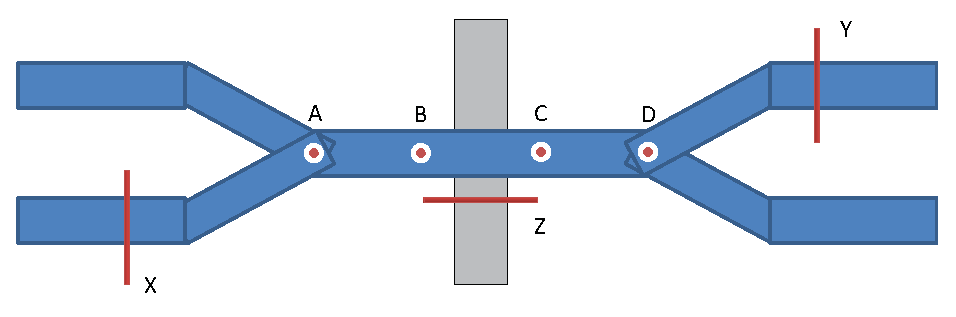
\includegraphics[width=\columnwidth]{diagramas/problema}
\caption{Planteamiento del problema}
\label{fig:problema}
\end{figure}

El entronque de tren está representado por las líneas azules, mientras que la vía de automóviles está representada por el rectángulo gris.
El sistema contará con cuatro sensores sobre la vía del tren, marcados con las letras A, B, C y D. Los sensores detectan la presencia del tren: se encuentran activos siempre que existe un tren encima de ellos.
Los sensores A y D se colocan en las entradas del segmento común de vía del entronque ferroviario, los sensores B y C se encuentran alrededor de la autovía.
También se instalarán barreras motorizadas (una a cada entrada del entronque y una más sobre el crucero), marcadas X, Y y Z.
En particular, la barrera Z cuenta con una luz roja, y una bocina de alarma.

Los requerimientos son los siguientes:
\begin{itemize}
	\item Si un tren viajando de Oeste a Este aparece en el sensor A, se debe cerrar la barrera Y (para evitar que un tren viajando en dirección opuesta entre por ese extremo del entronque).
	Se debe cerrar también la barrera Z y encender la luz roja y la alarma.

	\item Cuando el tren haya pasado el sensor C, se levantará la barrera Z, se apagará la luz y la alarma, pero la barrera Y permanecerá cerrada.

	\item Cuando el último vagón del tren haya pasado el sensor D, se levantará la barrera Y.

	\item Si por alguna razón el tren se detiene entre los sensores A y B (antes del crucero), se deberá levantar la barrera Z, apagar la sirena y poner la luz en intermitencia.
	Cuando el tren reanude su marcha, se debe cerrar nuevamente la barrera Z, dejar la luz encendida y activar la alarma.
	Evidentemente, la barrera Y permanece cerrada en esta situación.

	\item Un funcionamiento análogo ocurre si un tren viajando de Este a Oeste entra en el entronque.
\end{itemize}


\subsection{Descripción del SE utilizado}
\label{sub:metodologia-descripcion-SE}

De nueva cuenta ha sido utilizado el kit de Lego NXT MindStorms\footnote{http://www.legomindstorms.com/} habilitado con la arquitectura mostrada en la Figura \ref{fig:arquitectura-se-lego} que le permite comunicarse con el ambiente para recibir datos y ejecutar cálculos para producir la salida adecuada. Algunos de los componentes principales del kit Lego NXT son un procesador de 32 bits, una pantalla LCD, una interfaz de cuatro botones, tres actuadores (servomotores) y cuatro sensores (de contacto, de ultrasonido, micrófono y de luminosidad).

\begin{figure}[!t]
\centering
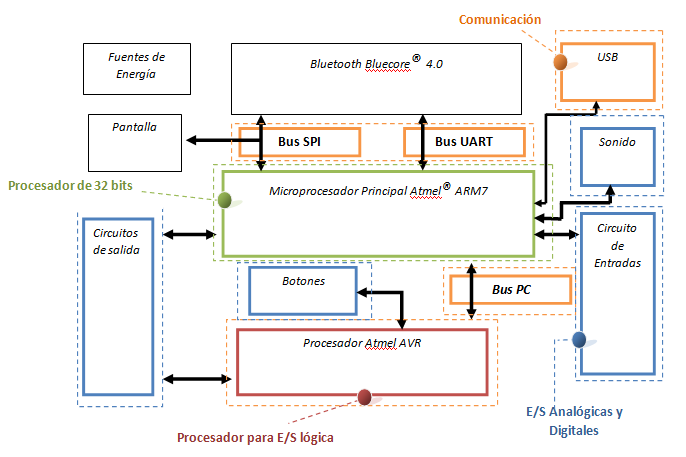
\includegraphics[width=\columnwidth]{diagramas/arquitectura-lego}
\caption{Arquitectura del SE del kit Lego NXT}
\label{fig:arquitectura-se-lego}
\end{figure}

El SE ha sido habilitado con tres actuadores (motores) que representan las tres barreras (X, Y, Z) presentes en el planteamiento del problema.
Cuatro sensores de contacto representan a los sensores A, B, C y D; finalmente la funcionalidad de alarma sonora y luz intermitente ha sido implementada directamente en la pantalla del dispositivo, esto debido a la limitación de tres salidas disponibles en el robot, lo cual impide que se añadan más elementos (actuadores) a los tres motores ya existentes en el problema.



La configuración final del SE es mostrada en la Figura \ref{fig:configuracion-lego}.

\begin{figure}[!t]
\centering
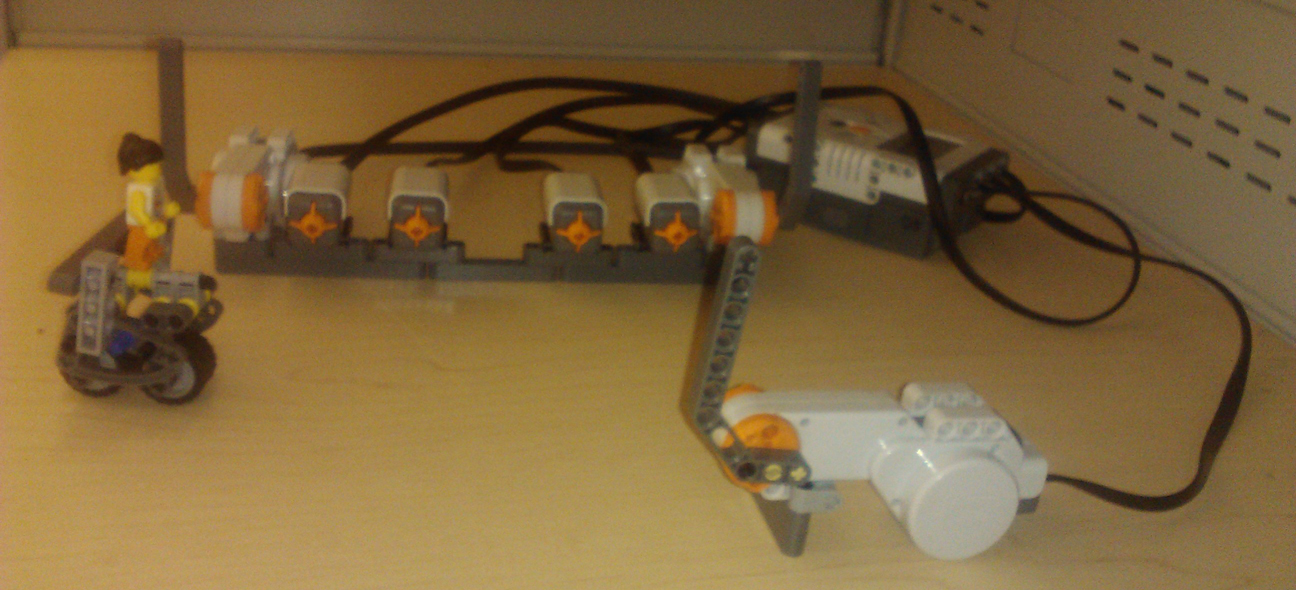
\includegraphics[width=\columnwidth]{diagramas/configuracion-lego}
\caption{Configuración del kit Lego NXT}
\label{fig:configuracion-lego}
\end{figure}

\subsection{Descripción de la implementación}
\label{sub:metodologia-modelado-statechart}

La descripción de la implementación puede ser abordada en dos partes, la primera comprendiendo el diseño y modelado del problema y la segunda referente a la codificación del diseño creado.

\vspace{0.5cm}
\textbf{\emph{Diseño del sistema}}

El diseño del sistema fue realizado contemplando un conjunto de cinco estados.
Cada uno de ellos representa una situación en el sistema e internamente se encuentra por la escucha a una o más señales y posteriormente el desencadenamiento de un comportamiento específico, seguido por el \emph{envío} a un nuevo estado.

La Figura \ref{fig:estados-modelo} muestra los diagramas Statecharts de los estados diseñados, los cuales también son descritos a continuación:
\begin{itemize}
	\item \emph{\textbf{Inicial (Start, Subfigura \ref{fig:estado-Start}):}} En primera instancia detecta la pulsación de alguno de los sensores A o D.
	La identificación individual permite detectar si el tren entra por la izquierda o por la derecha.
	Una vez hecha esta detección es posible reconfigurar el resto de los estados para que tengan el comportamiento adecuado (levantar o bajar las barreras y escuchar a los sensores convenientes).
	Luego, se realizan las actividades físicas que involucran que el carril del auto se encuentre cerrado, esto es bajar la barrera del carril del auto, la barrera del tren del lado contrario y encender la luz y la alarma.
	Finalmente, se establece un temporizador para detectar el caso en el que el tren se detenga entre los sensores A y B y se envía al sistema al estado Carril Auto Cerrado.

	\item \emph{\textbf{Carril Auto Cerrado (CAC, Subfigura \ref{fig:estado-CAC}):} } Una vez que el estado del sistema refleja que el carril del auto está cerrado, este estado escucha a dos eventos, la pulsación del sensor B o el fin del temporizador establecido en el estado Inicial.
	Si el temporizador llega a su fin, el tren se ha quedado entre los sensores A y B, por lo que se desencadenan las tareas relacionadas con el estado de Carril Auto Precaución, esto es, abrir la barrera Z, encender la luz intermitente y apagar la alarma; el sistema se envía al estado Carril Auto Precaución.

	Por el contrario, si el sensor B es presionado, para este caso en específico significa que el tren no se ha detenido y dado que la barrera y el resto de elementos (alarma, luz) tienen ya el comportamiento adecuado asignado, no se realiza acción nueva alguna, únicamente se traslada al sistema al estado Tren En Medio.

	\item \emph{\textbf{Carril Auto Precaución(CAP, Subfigura \ref{fig:estado-CAP}):}} Como se ha mencionado, este estado se origina cuando el temporizador lanzado en el estado Inicial alcanza su fin.
	Este estado espera la pulsación del sensor B para llevar volver a encender la luz, bajar la barrera Z y llevar al sistema al estado de Tren En Medio.

	\item \emph{\textbf{Tren En Medio (TEM, Subfigura \ref{fig:estado-tem}):}} Después de que el tren se encuentra posicionado entre los sensores B y C, este estado espera la pulsación del sensor C para realizar el conjunto de tareas que denotan que el carril del auto ha sido reabierto, esto es levantar la barrera Z, apagar la luz y apagar la alarma.
	Finalmente, lleva al sistema al estado Carril Auto Reabierto.

	\item \emph{\textbf{Carril Auto Reabierto (CAR, Subfigura \ref{fig:estado-CAR}):}} Cuando el tren se ubica entre los sensores C y D, este estado espera que el sensor D sea presionado y liberado para realizar el conjunto de tareas que denotan que el tren ha salido del sistema, esto es levantar la barrera Y.
	Finalmente, se envía al sistema de nueva cuenta al estado Inicial para la detección de más trenes aproximándose al cruce.
\end{itemize}

\begin{figure*}[!t]
\centering

\subfigure[Start]{
	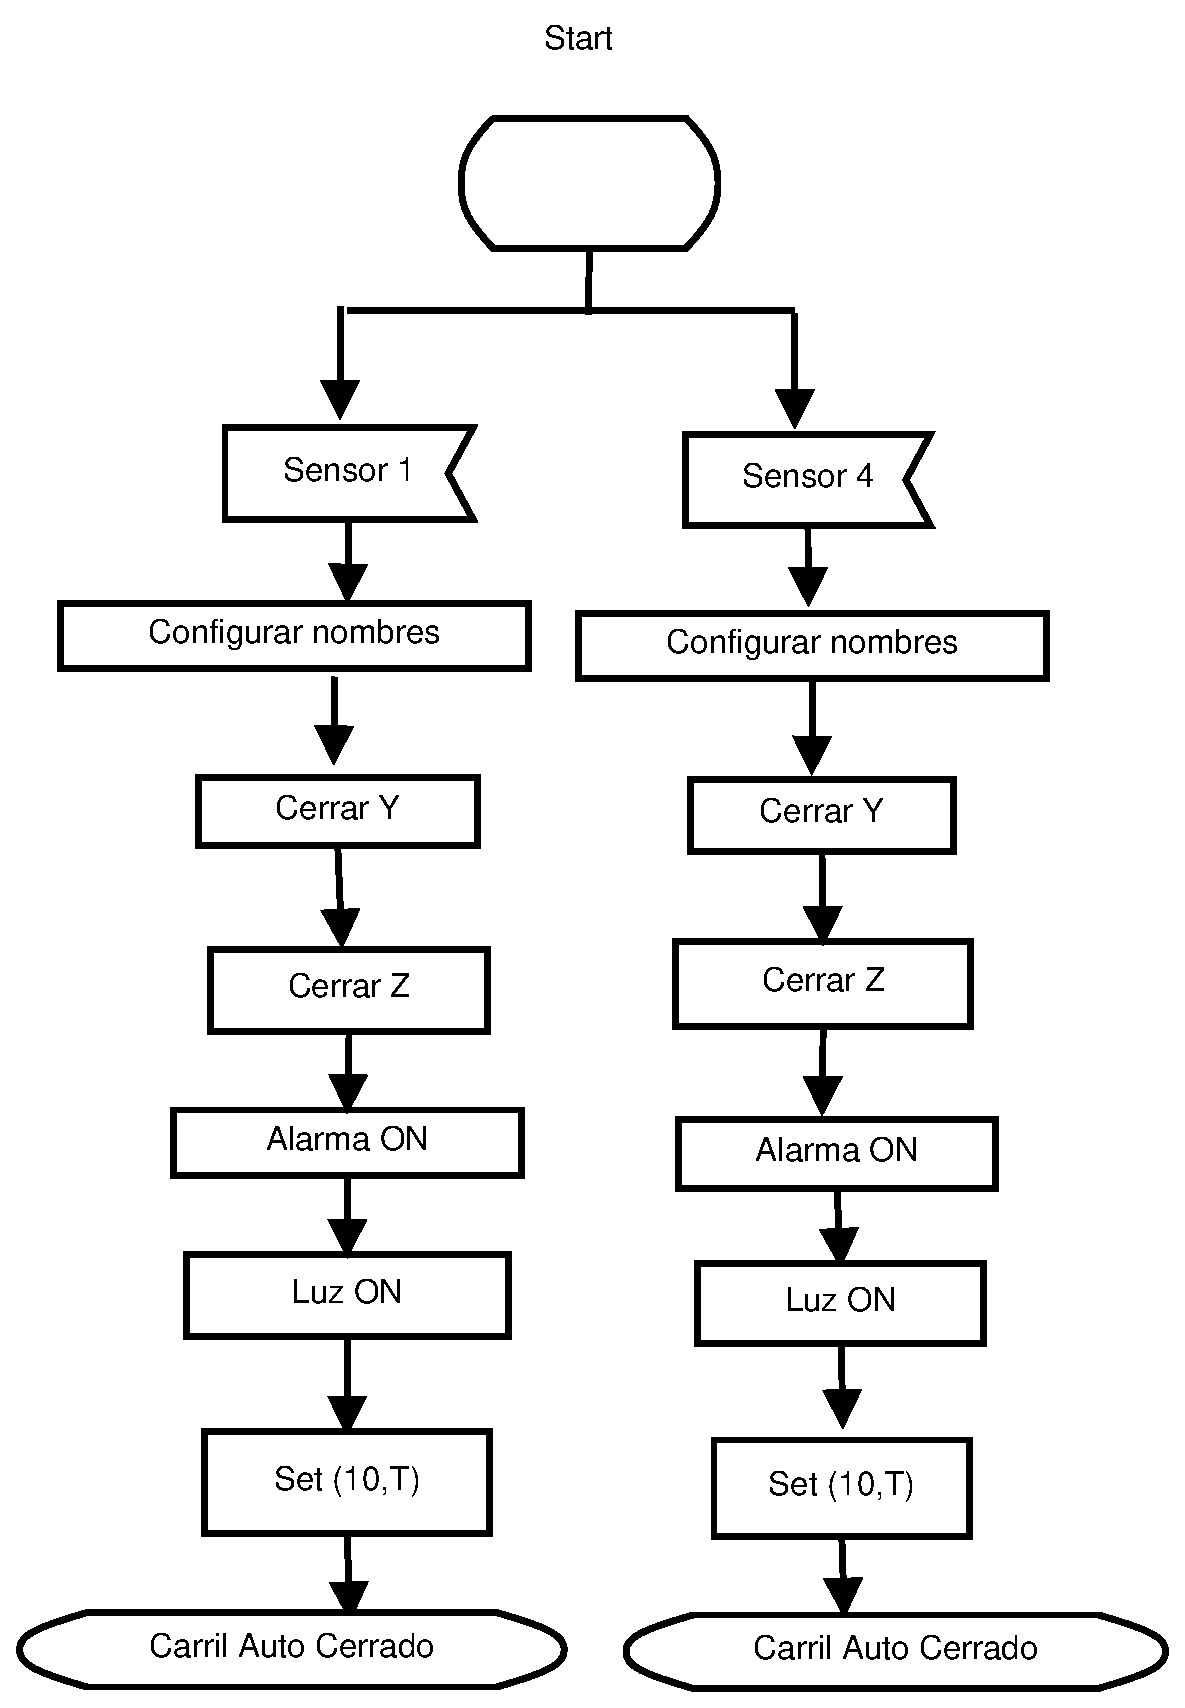
\includegraphics[width=0.25\textwidth]{diagramas/Start}
	\label{fig:estado-Start}
}%\qquad
\subfigure[Carril Auto Cerrado]{
	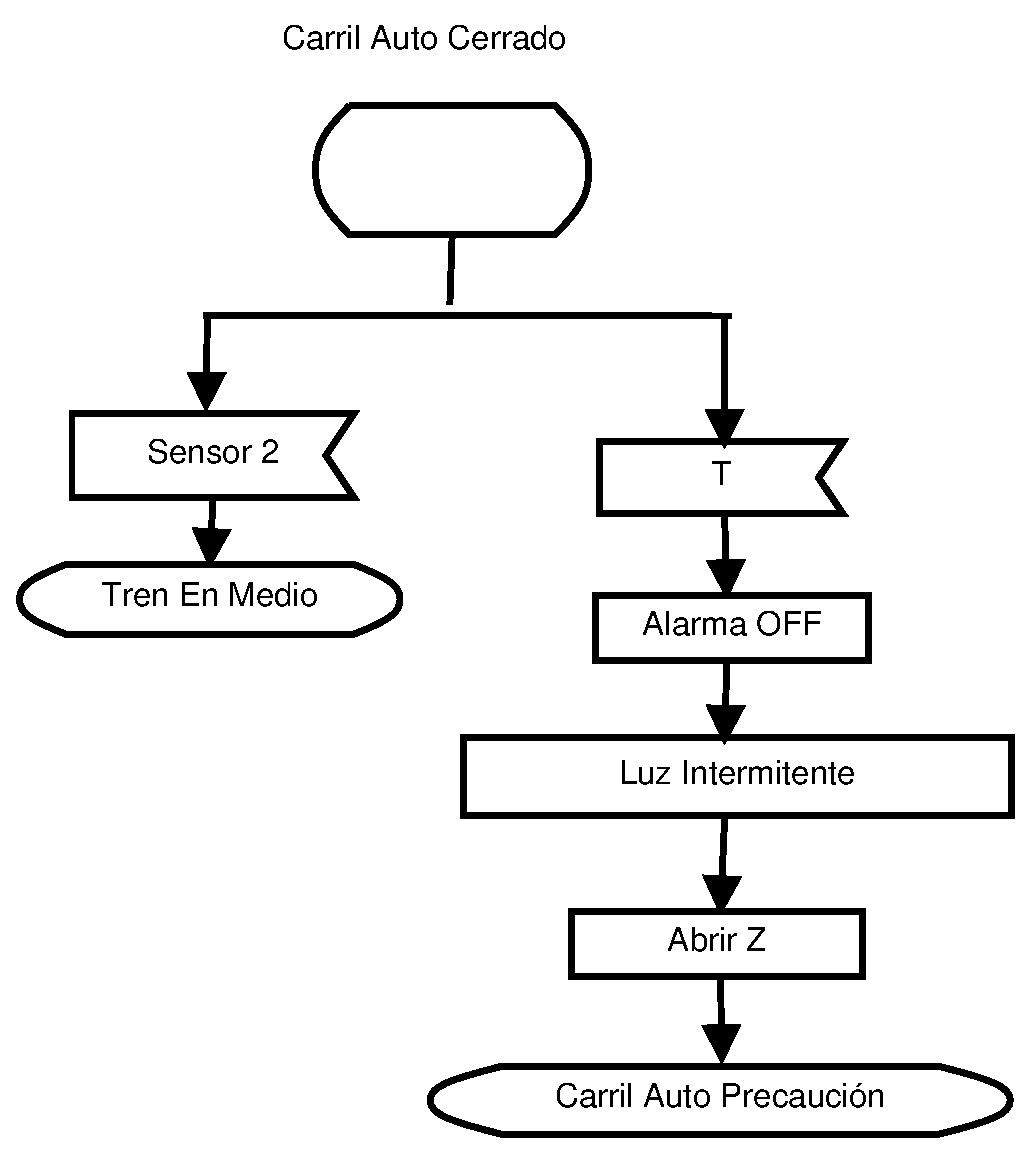
\includegraphics[width=0.25\textwidth]{diagramas/CAC}
	\label{fig:estado-CAC}
}
\subfigure[Carril Auto Precaución]{
   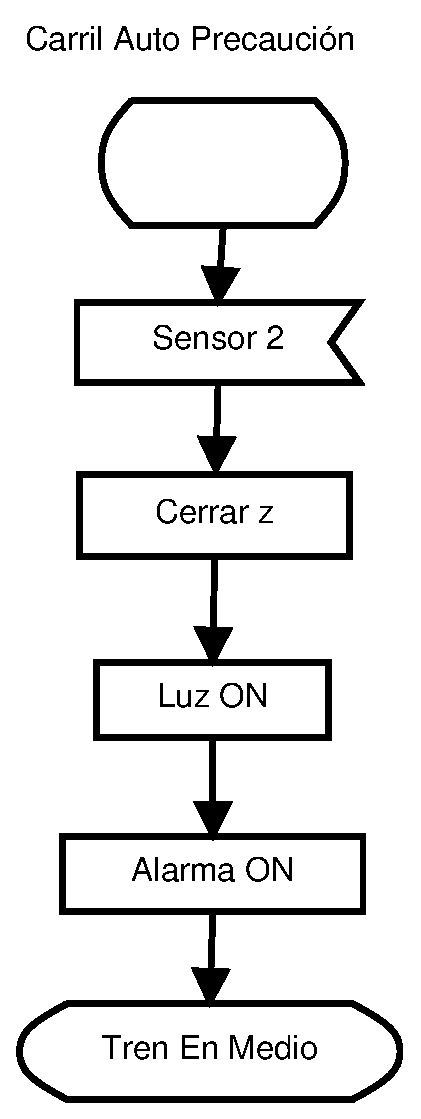
\includegraphics[width=0.1\textwidth]{diagramas/CAP}
   \label{fig:estado-CAP}
 }
\subfigure[Tren En Medio]{
   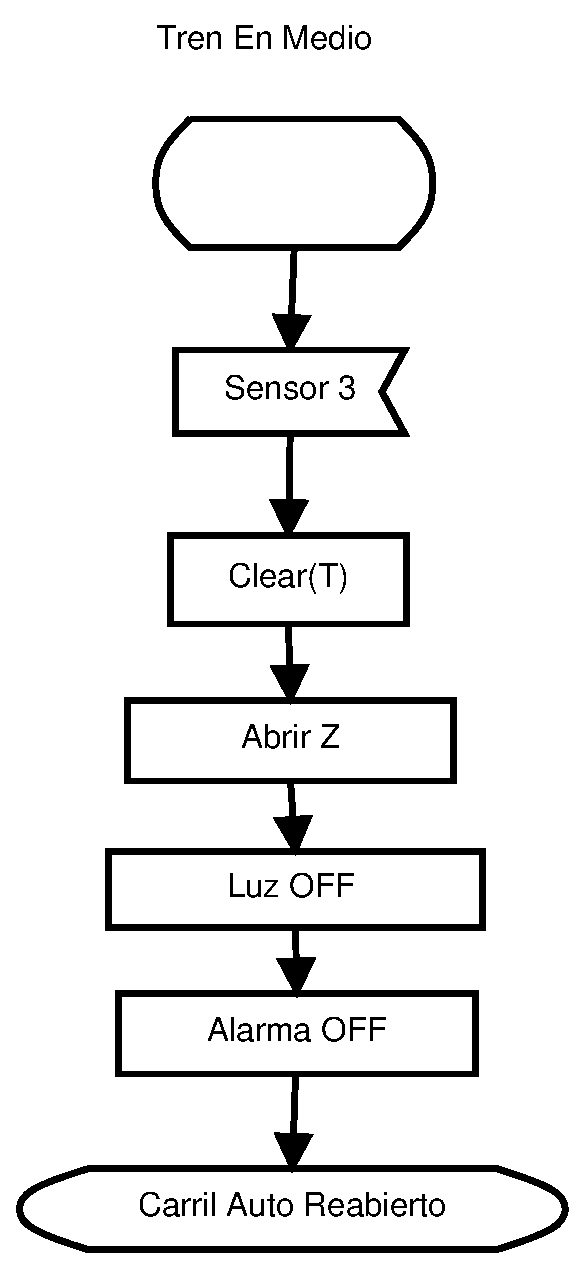
\includegraphics[width=0.15\textwidth]{diagramas/TEM}
   \label{fig:estado-tem}
}
\subfigure[Carril Auto reabierto]{
   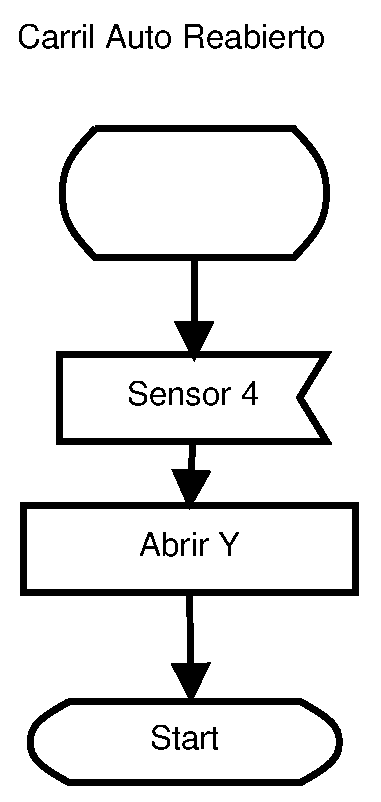
\includegraphics[width=0.1\textwidth]{diagramas/CAR}
   \label{fig:estado-CAR}
 }

\subfigure[Diagrama global]{
   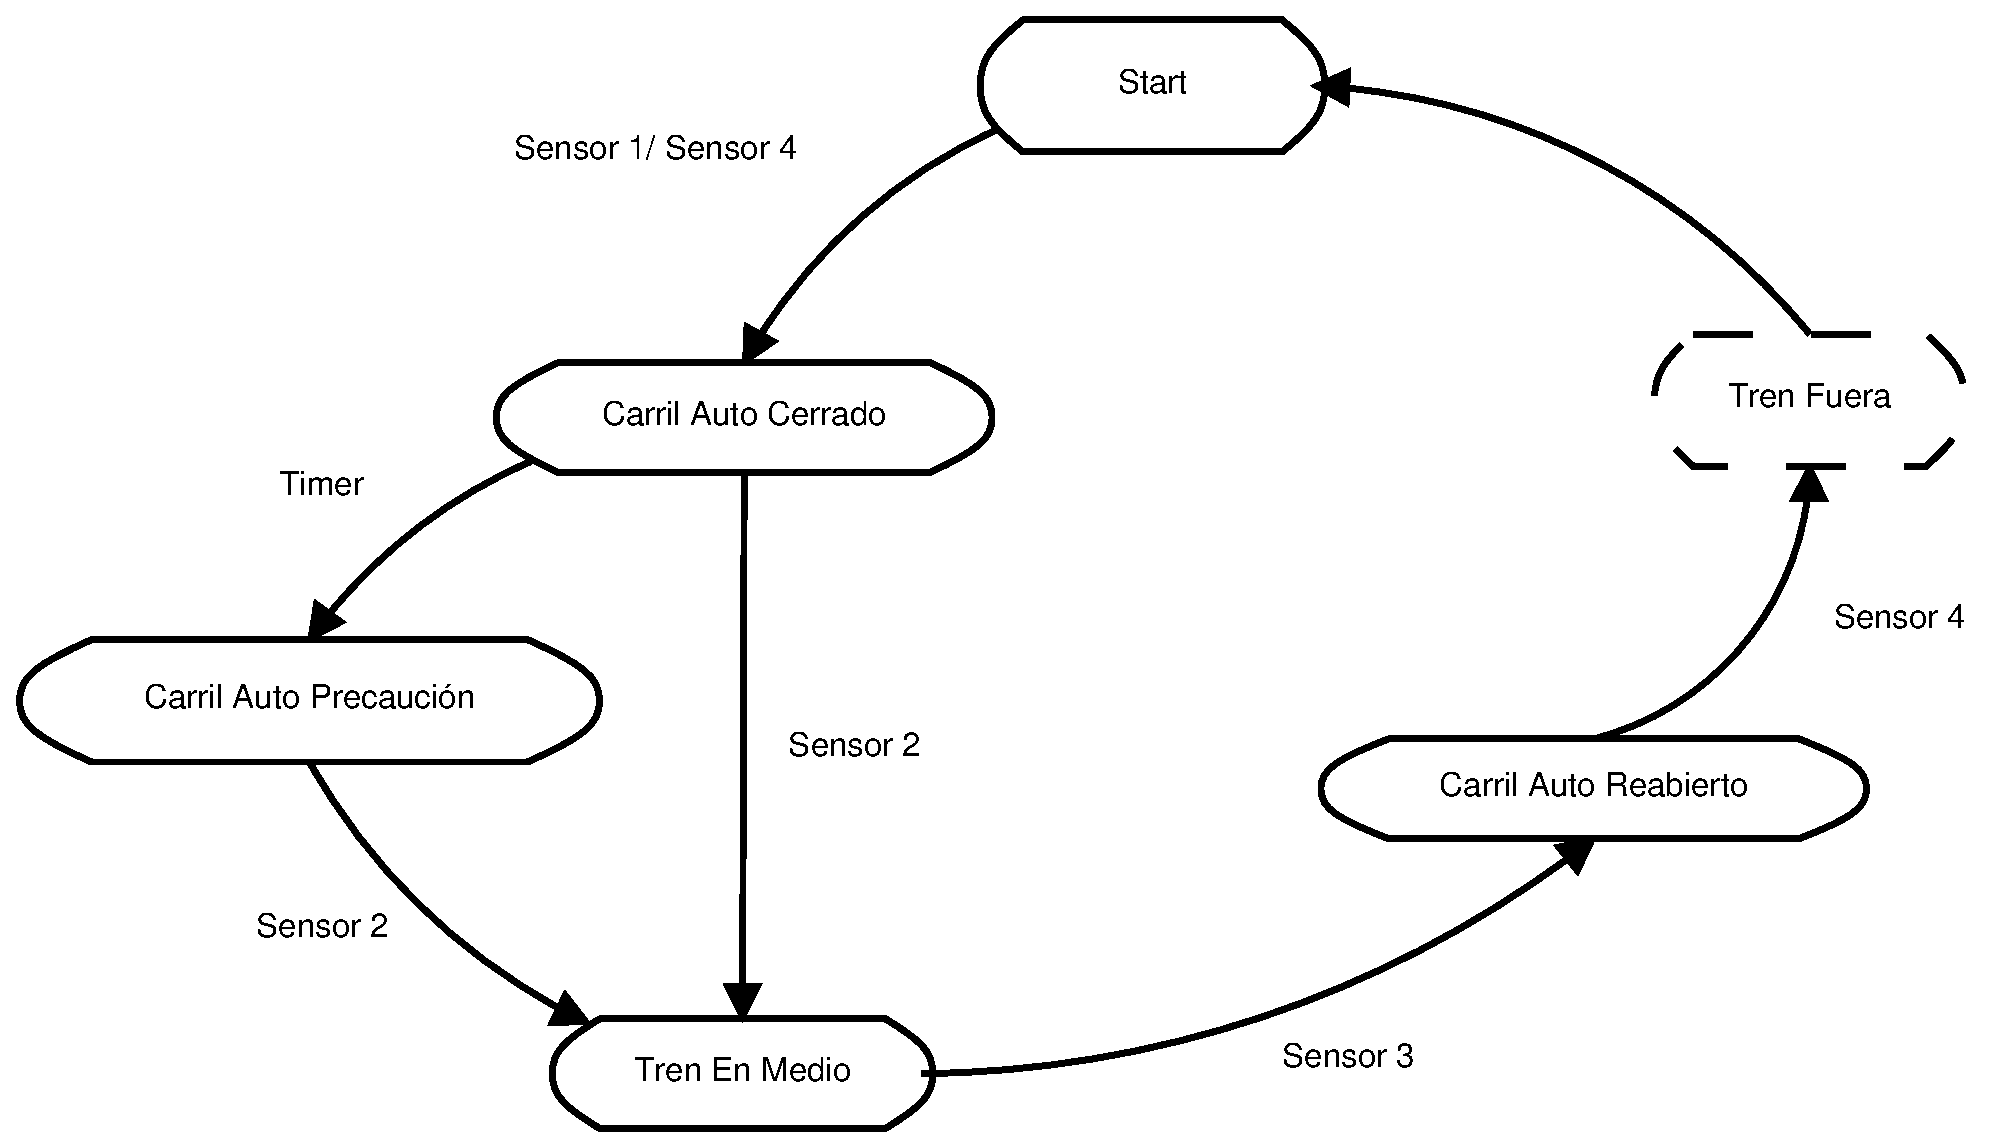
\includegraphics[width=0.7\textwidth]{diagramas/global}
   \label{fig:estado-global}
 }
\caption{Estados del modelo propuesto}
\label{fig:estados-modelo}
\end{figure*}

\vspace{0.5cm}
\textbf{\emph{Codificación del diseño}}

Debido a que la elaboración del diseño utilizando Statecharts se manifiesta como una máquina de estados finitos, el pseudocódigo de la implementación refleja un bucle infinito con un bloque \emph{switch} embebido, el cual contiene en cada uno de sus \emph{case’s} a los estados previamente descritos.

\begin{algorithm}
\begin{algorithmic}[1]

\STATE $t_{inicial} = 0$ (inicio del timer).
\STATE $t_{consumido} = 0$ (tiempo consumido desde inicio timer)
\STATE $t_{maximo} = 0$ (umbral para considerar tren estacionado)
\STATE $s_{final} = $ \FALSE (último sensor pulsado)
\WHILE {\TRUE}
	\SWITCH{$s$}
		\CASE{INICIAL}
			\IF{SENSOR\_1 \OR SENSOR\_4}
				\IF{SENSOR\_1}
					\STATE trenPorIzquierda = \TRUE
				\ELSE
					\STATE trenPorIzquierda = \FALSE
				\ENDIF
				\STATE ejecutar tareasCarrilAutoCerrado()
				\STATE $t_{inicial}$ = CurrentTick()
				\STATE estado = CAC
			\ENDIF
	    \ENDCASE

	    \CASE{CAC}
	    	\STATE $t_{consumido}$ = CurrentTick() - $t_{inicial}$
           	\IF{$t_{consumido} > t_{maximo}$}
              \STATE ejecutar tareasCarrilAutoPrecaucion()
              \STATE estado = CAP
           	\ENDIF

           	\IF{SENSOR\_2}
           		\STATE ejecutar tareasTrenEnMedio(false)
           		\STATE estado = TEM
            \ENDIF
	    \ENDCASE

	    \CASE{CAP}
	    	\IF{SENSOR\_2}
	    		\STATE ejecutar tareasTrenEnMedio(true)
	    		\STATE estado = TEM
	    	\ENDIF
	    \ENDCASE
	    
	    \CASE{TEM}
	    	\IF{SENSOR\_3}
	    		\STATE ejecutar tareasCarrilAutoReabierto()
	    		\STATE estado = CAR
	    	\ENDIF
	    \ENDCASE

	    \CASE{CAR}
	    	\IF{SENSOR\_4}
	    		\STATE sensorFinal = \TRUE
	    	\ENDIF

	    	\IF{$s_{final}$ = \TRUE \AND SENSOR\_4 = \FALSE}
	    		\STATE $s_{final}$ = \FALSE
	    		\STATE ejecutar tareasTrenFuera()
	    		\STATE estado = Inicial
	    	\ENDIF
	    \ENDCASE

    \ENDSWITCH
\ENDWHILE

\end{algorithmic}
\caption{Pseudocódigo de la implementación realizada}
\label{alg:pseudocodigo}
\end{algorithm}

En Pseudocódigo \ref{alg:pseudocodigo} se muestra el pseudocódigo del SE, ilustrando el bloque \emph{switch} y la navegación entre sus estados.
Como puede notarse, la llamada a \texttt{tareasTrenEnMedio()} incluye un parámetro booleano que indica si las tareas deben ejecutarse considerando que el estado anterior es el de Carril Auto Precaución o no, esto debido a pequeñas diferencias que deben ser observadas en su implementación.
Adicionalmente, es oportuno indicar que las lecturas de los sensores (SENSOR\_1, SENSOR\_2, etc.) son reacondicionadas para leer el sensor adecuado dependiendo de la dirección del tren que ingresa a las vías.


\section{Resultados} 
\label{sec:resultados}
Después de la realización de pruebas con el sistema implementado, se han obtenido resultados satisfactorios, por lo que el sistema se comporta de acuerdo a lo establecido en los lineamientos iniciales.

La única situación no abordada se refiere a la integración de una luz física como tal, esto debido a que el kit Lego solamente contiene tres salidas de potencia, las cuales ya se encontraban ocupadas por los tres motores que controlan a las barreras.
Debido a esta razón, el estado de la luz fue mostrado únicamente en la pantalla del robot.
Se probó además que el tren abordara tanto por la izquierda como por la derecha, obteniendo también resultados satisfactorios.


\section{Discusión y conclusiones}
\label{sec:discusion}
A pesar de la aparente sencillez de la actividad realizada, es importante notar que resultó un buen reto para mejorar las capacidades de diseño y modelado de sistemas.
La perspectiva del diseño de sistemas de este tipo es muy distinta a la observada en la construcción de \emph{software clásico}, ya que hay un especial interés en la obtención de los elementos que van a participar en el sistema y su interacción, a diferencia del software clásico en el que lo que normalmente se busca es la obtención e implementación de un algoritmo a modo de serie de pasos para lograr un requisito establecido desde el análisis.

Como un comentario final, nos ha parecido relevante el hecho de que después de contar con el modelo y haber reconocido que la cobertura ante los escenarios descritos era la adecuada, la implementación (codificación) del SE resultó sencilla y se aceleró de forma considerable.
Se ha comprobado que dedicar tiempo y esfuerzos en un buen análisis utilizando la herramienta adecuada ayuda a obtener una descripción del sistema completa, fácil de entender y que ofrece baja complejidad al momento de ser codificada.

\bibliographystyle{plain}
\bibliography{bibliography/references}
\end{document}